\section{Architectural Decisions}
\label{se:architectural_decisions}

Initial design of \acrshort{wdias} used the \acrfull{soa}. Moreover, it tried to use an \acrfull{esb} to integrate different modules, as \acrshort{esb} is acting as a common layer for all of modules. By default, \acrshort{esb} also provides publisher/subscribe (pub/sub) capabilities.
\hl{Because} \acrshort{esb} \hl{mediator can be used to integrate the modules which are described in Section} \ref{subse:modules_weather_data_integration_sys}. 
\gkc{FIXED}
The \acrshort{esb} has the processing units called \emph{mediators}. A mediator can take a message, carry out some predefined actions on it, and output the modified message. This mediator capabilities can use to integrate the modules of a weather data system as shown in \cref{fi:wdia_components}. \acrshort{esb} also support different transportation protocols such as HTTP and Web sockets. However, it turned out that \acrshort{esb} is not a suitable for data streaming or bulk data processing. Also, \acrshort{esb} suffer from single point of failure, as all the messages are going though a common bus and slower communication (can’t use for transfer data).

In the second design phase of \acrshort{wdias}, we attempted to use the actor model using AKKA framework \cite{HewittWhyModel} in order to overcome above \acrshort{esb} drawbacks. At the same time, we moved away from the \acrshort{soa} architecture design to the microservice architecture design. Thus we redesign the system architecture with decompose into microservices and used actors to implement each microservice in the system. In that case, an actor or an actor with slave actors were map to each microservice in \acrshort{wdias}. \acrshort{soa} focuses on imperative programming, whereas microservices architecture focuses on a responsive-actor programming style using faster messaging mechanisms. 

When compare to \acrshort{soa}, the microservice architecture has several advantages such as the following:
\begin{itemize}
    \item Follow the Single Responsibility principle
    \item Resilient/flexible as failure in one service does not impact other services. If you have monolithic or bulky service errors in one service/module it can impact other modules/functionality.
    \item High scalable as demanding services can be deployed in multiple servers to enhance performance and keep away from other services so that they do not impact other services. Will be difficult to achieve the same with single, large monolithic service.
    \item Easy to enhance as dependencies are less. Is also easier to change and test.
    \item Low impact on other services as each service is independent. % service., this has less chance to impact other services
    \item Easy to understand since they represent a small piece of functionality
    \item Ease of deployment
\end{itemize}

% /hl{The typical \acrshort{soa} model, for example, usually has more dependent \acrshort{esb}s, with microservices using faster messaging mechanisms. \acrshort{soa} also focuses on imperative programming, whereas microservices architecture focuses on a responsive-actor programming style.}
\dbc{Multiple design rounds and decisions are mixed in the para. First finish discussing ESB. Then finish actor model in another para. Then focus on mircoservice details.}

Even with using the AKKA framework, it has some of the disadvantage with implementing each microservice as an actor as described in AKKA documentation \cite{Akka.ioWhenCluster}. One of the attractive feature of microservice architecture is independent nature of the microservices. This allows to choose a different technology for each microservice based on the advantage that could bring in. Also allowed to independently develop and maintain by multiple smaller and more focused teams/communities. But using the actors as microservice, the actors messaging between different services cause to result in a too tight code coupling between the services and difficulties deploying these independent of each other, which is one of the main reasons for using a microservices architecture \cite{Akka.ioWhenCluster}. To overcome these issues, we moved to the concept of container-orchestration based architecture.

\dbc{Kubernetes is a product. What you need to refer is to the concept of container-orchestration. Fix.}

% \begin{itemize}
%     \item \hl{Unable to choose technology. But} \acrshort{k8s} \hl{allows you to choose technology that is best suited for a particular functionality}
%     \item \hl{As mentioned in the AKKA documentation} \cite{Akka.ioWhenCluster}, \hl{it is better for developing one microservice within the whole} \acrshort{wdias} design.
% \end{itemize}

\dbc{What are these 2 bullets?}
\gkc{Absorbed those two points into above paragraph}
\dbc{Don't use shortened words like it's, isn't, don't,... in writing}

%%%%%%%%%%%%%%%%%%%%%%%%%%%%%%%%%%%%%%%%%%%%%%%%%%%%%%%%%%%%%%%%%%%%%%%%%%%%%%%%
% \subsection{Brief introduction to the \acrfull{k8s}}
% \label{sebse:k8s_intro}

Containerization is an alternative to the virtualization that supports via virtual machines or Hypervisors. It involves encapsulating or packaging up software code and all its dependencies so that it can run uniformly and consistently on any infrastructure \cite{IBMContainerizationExplained}. The concept of containerization and process isolation is emerged after the open source Docker Engine \cite{DockerAppContainerization}, an industry standard for package software into standardized units for development, shipment and deployment.

\acrfull{k8s} is an open-source system for automating deployment, scaling, and management of containerized applications \cite{LinuxFoundationProduction-GradeKubernetes}. It groups containers that make up an application into logical units for easy management and discovery. While implementing the \acrshort{wdias}, we used \acrshort{k8s} as the container-orchestration system, in order to deploy each microservice as container and manage with providing scalability and availability.

\begin{figure}[htp]
    \centering
    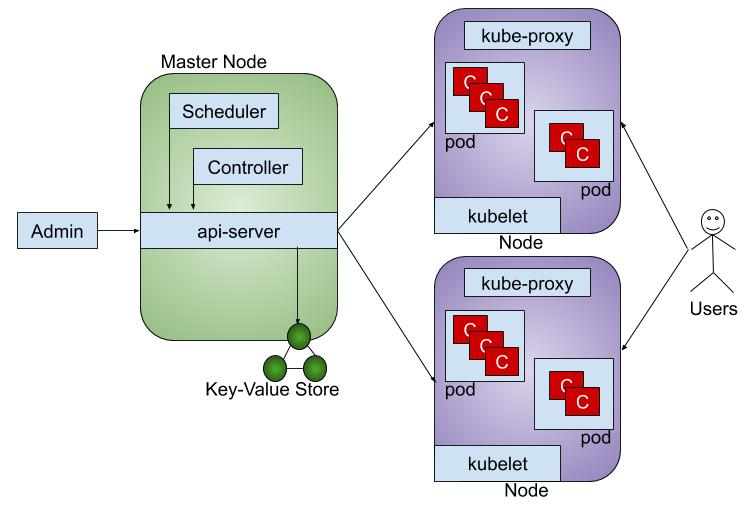
\includegraphics[width=1\textwidth]{method/microservice/k8s_architecture_v3.jpg}
    \caption{\acrfull{k8s} architecture.}
    \label{fi:k8s_architecture}
\end{figure}
\cref{fi:k8s_architecture} gives an overall idea on the components of \acrshort{k8s},
\begin{itemize}
    \item Pods -- Cluster of containers that can group other container images in a single unit.
    \item Nodes -- the machines (VMs, physical servers, etc) in a cluster that run your applications and cloud workflows.
    \item kubelet -- An agent that runs on each node in the cluster. It makes sure that containers are running in a pod.
    \item kube-proxy -- A network proxy that runs on each node in the cluster, and maintains network rules on nodes.
    \item Kubernetes master -- Responsible for maintaining the desired state for your cluster.
    \item etcd -- Consistent and highly-available key value store used as Kubernetes’ backing store for all cluster data.
\end{itemize}

Users can add much as required Nodes into the \acrshort{k8s} cluster, and \acrshort{k8s} manage and deploy application as pods into cluster nodes.
Each microservice can deploy as a Pod which is a group of containerize applications. And \acrshort{k8s} able to scale as much as user want as described above.
By separating each microservice as a container, and running them as multiple pods inside the \acrshort{k8s} removes the tight coupling of microservices when compared to the actors. This preserves the independent nature of the microservices which allows to high scale the system.
